%!TEX root=../main.tex
\chapter{Climbing Mont Blanc Usability Goals}
\label{ch:design}
This chapter starts with a definition of usable software systems in \Cref{sec:usability-def}. The section will define usability, and show a few aspects and characteristics in other \glspl{oj} which makes them usable with respect to the definition presented. \Cref{sec:cmb-usability} ends the chapter with a discussion of the importance of the usability goals set by this thesis.

\section{Usability in Online Judge Systems}
\label{sec:usability-def}
Usability is defined in the ISO 9241 standard Part 11 \cite{ISO1998} as ``the extent to which a product can be used by specified users to achieve specified goals with effectiveness, efficiency, and satisfaction in a specified context of use.'' The definition is broad and covers many aspects of a product, or in our case a software system. Usability is a broad term and can be hard to define precisely, however, literature seems to agree that the following five characteristics describe a usable software system  \cite{holzinger2005, ferre2001}; \textit{learnability}, \textit{efficiency}, \textit{user retention over time}, \textit{error rate}, and \textit{satisfaction}. A quick summary of each characteristic is summarized below.

\paragraph*{Learnability:} The users ability to learn to use the system. Learnability also involves the users ability to gain efficiency in using the system and reach their objectives in a quick manner.

\paragraph*{Efficiency:} Users should be allowed to obtain a high level of productivity when using the system. The usability is improved if the user can quickly reach their goals when using the system.

\paragraph*{User Retention Over Time:} The user should be able to return to the system after a break from using it, and remember the core functionality of the system. A usable software system makes it easy to get back into an efficient state without the need to learn the core functionality of the system a new. The characteristic is also refered to as \textit{memorability}.

\paragraph*{Error Rate:} The number of errors a user makes along the path of actions before reaching his or hers goal. A low error rate among users improves the usability of the system.

\paragraph*{Satisfaction:} The users subjective thoughts about the system as well as making the system pleasant to use. Satisfaction may involve functionality that is both visible and invisible through the system frontend.\\

Another related term to system usability is the notion of \textit{affordance} of things, which is described by Donald Norman:
\blockquote{``...the perceived and actual properties of the thing, primarily those fundamental properties that determine just how the thing could be used [..] Affordances provide strong clues to the operations of things. Plates are for pushing. Knobs are for turning. [..] Complex things may require explanation, but simple things should not. When simple things need pictures, labels, or instructions, the design has failed.''  \cite{norman1988design}}

Good affordances of entities and components in software systems will improve learnability, efficiency, memorability, and user satisfaction while lowering error rates, and thereby improve the usability of the system. \\

The definition of \glspl{oj} as presented in \Cref{sec:related} is quite straightforward. However, because of its simplicity, it is fairly important that the \gls{oj} is highly usable when users are actively using the system to solve programming problems. The most time-consuming tasks done by most users in an \gls{oj}, at least in the \gls{cmb} system, is to read problem descriptions as well as submit code for automatic judgement. The time spent on reading and submitting is minimalistic compared to the time spent on developing code, and code development often happen off site in an offline environment if not explicitly offered by the \gls{oj}\footnote{Some of the mentioned \glspl{oj} has web based code editors, such as Kattis \cite{KATTIS} or HackerEarth \cite{HACKEREARTH}}. \\

The action of uploading code is one of the main actions done by users. Making the action of uploading code simple is important for both efficiency and learnability. \glspl{oj} like HackerEarth makes it easy to upload code, providing an online code editor which can compile and test the code or directly submit a solution like shown in Figure \ref{fig:hackerearth-upload}. The user also has the option of uploading source files directly, which makes it easier for the users wanting to submit source files instead of coding directly in the browser. Presenting multiple alternatives in a structured way to users makes it simpler to use the system, as a given user may choose the method he or she is most comfortable with. The upload feature also shows good affordance, and the user knows by instinct how to submit code. \\

\begin{figure}
    \centering
    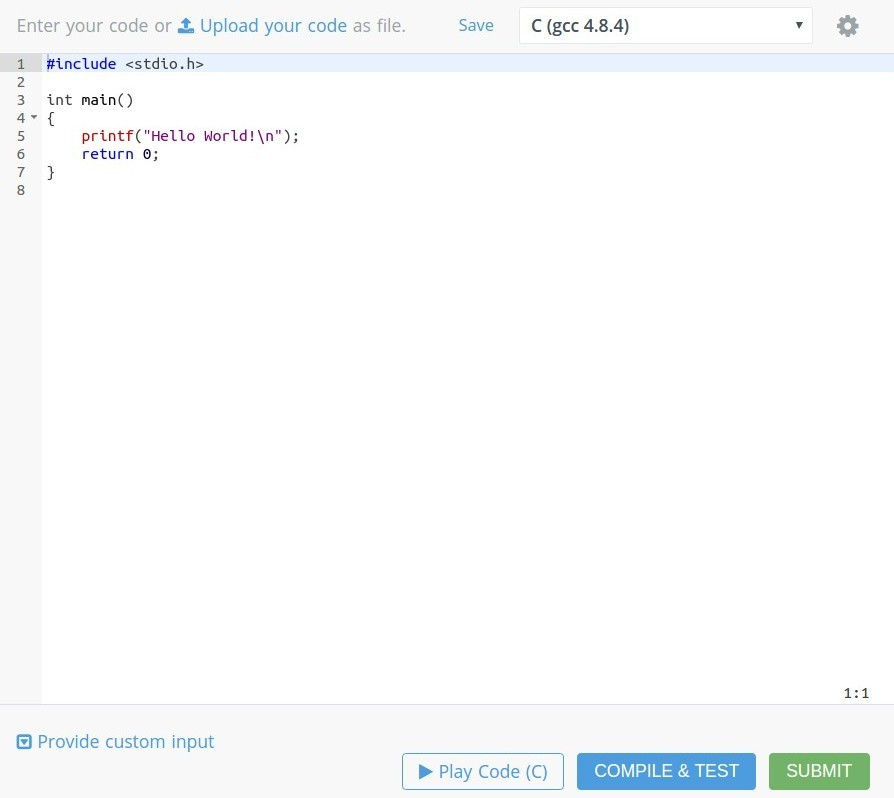
\includegraphics[width=0.8\textwidth]{figs/hackerearth_upload.jpg}
    \caption[HackerEarth Code Upload]{HackerEarth Code Upload (source: HackerEarth Website \cite{HACKEREARTH})}
    \label{fig:hackerearth-upload}
\end{figure}

It is also important that the user gets feedback on the state of submitted program. Tracking the state and repeatedly report to the user whenever the state of the submission changes is critical. It does not have to be very detailed, as long as the user get some notion of the state of the program. For example, Kattis does not automatically report the state of a submitted program, but they display a type of progress bar which is updated whenever test cases pass, and the user manually refreshes the current view. However, the more information displayed about critical data such as the state of the submission, the better. \\

The different components in the user interface should also respond as expected and give logical feedback. Failing to do so might distract the user, and thereby blocking the user from reaching his or hers goal. Norman mentions in his book that it is important that all actions made against the system should ``give an immidiate and obvious effect'' in the form of feedback to the users \cite{norman1988design}. For \glspl{oj}, this means clearly stating feedback and making the feedback visible for the users, as well as presenting useful and descriptive feedback messages.\\

Administrator users is also a part of the user group. Usability in \glspl{oj} also involves making the system usable for system administrators and problem makers, and it is important that admin interface usage is simple and understandable. Usage of a given admin interface likely require some training and knowledge about the system, but the interface should be simple, so users do not have to relearn how to use the system and quickly achieve high efficiency, i.e. high user retention over time. \\

Other features implemented by the judge should also behave as expected and the interface should be logically built. The \glspl{oj} presented in chapter offers various features and going into depth about the usability of this features is outside the scope of this thesis. However, it is worth mentioning that the \glspl{oj} should build the system with components with good affordances as described above. The professional \glspl{oj} mentioned in \Cref{sec:related} all have teams of developers and designers and offer simple and usable interfaces for their judges.

\section{Climbing Mont Blanc Usability Goals}
\label{sec:cmb-usability}
% Dra inn målene presentert i kapittel 1, og si motivasjonen til at det blir implementert med hensyn på seksjonen over.
% Ease of use + performance + quick response + feedback
\Cref{sec:ps-inter} presented the usability goals for this thesis. The listed usability objectives was chosen as the objectives are important for system usability, as well as some features potential for future development of the \gls{cmb} prototype. This section further elaborates on the objectives' importance, achored in the theory presented in the above section and to some extend the features' potential for future development of the system. \\

The objective \texttt{U1} concerns the bugs and known issues when starting this thesis in January of 2016, and is devided into three sub-objectives. Fixing bugs and known issues is important and, in some cases, crucial to offer a system with good usability. Making it possible for Mac OS X users to upload code to the system, i.e solving objective \texttt{U1.1}, is crucial for usability in the \gls{cmb} system. If users are denied uploading to the system even with a seemingly correct zip-file, it is likely that their satisfaction over the system will be low. As the \gls{cmb} team aims to offer the \gls{oj} to as many people as possible, with support for the major operating systems and browsers, it is therefore unacceptable to deny users using Mac OS X access to the system. \\

Submissions should not be able to block execution on the board and be locked in a running state i.e objective \texttt{U1.2}. The bug does not only give poor feedback to the user who submitted the problem, it does also block other users from using the system. The efficiency and satisfaction of other users trying to use the system would likely be low, as they are not given any feedback on the situation. The last issue concerns showing hidden submissions upon sorting on different highscore list metrics i.e objective \texttt{U1.3}, and is considered a nice-to-have fix and is less crucial compared to the other issues presented here. However, it does effect the general satisfaction with the system and it may increase the error rate and confusion of some users. \\

The objective \texttt{U2} is concerned with further extending the system with usability features. The five usability sub-objectives aims to further improve or extend the usability of the system, either by adding new features or enhance existing system components. The objective \texttt{U2.1} aims to better the feedback presented to users by making feedback more structured, clear, and visible especially during error messages. Immidiate and obvious feedback is, as mentioned before, important and it may help users gain efficiency and better the users learnability of the system. This due to every action giving obvious and immidiate feedback, which helps users acheive their goals. Actions who requires time to finish execute, such as running submissions, should give some feedback on the state of the action. Preferably, some feedback should also be given to indicate when the action is done executing. \\

Implementing real-time updates of data is related to giving good feedback and is the goal of objective \texttt{U2.2}. The feature makes it possible to automatically update the data displayed in the view, which for most users makes the system more satisfiable to use as they no longer need to manually update the web page to receive up to date data. It also displays good affordance, as users may expect the frontend views to change as data changes. The feature also has huge potential and can be used when further extending the system with more features. Some examples include detailed statistics of expected queue time and notifications when a submissions queue position changes. The \Cref{sec:future-work} mentions some possible future extensions which may use the real-time update technology in their implementation. \\

Newly added problems should be more stable and submissions to the problem should have a predictable outcome. This is covered by objective \texttt{U2.3}, and is important to both administrators and regular users. Administrators might become unsure of the functionality of the admin interface, and it also lowers satisfaction and increases the error rate on adding problems among system administrators. Users might begin to doubt their own, possibly correct, code depending on system output on the problem, which lowers efficiency and learnability while the error rates increases. \\

The last two objectives are mainly focused on user satisfaction. Objective \texttt{U2.4} aims to develop a bulletin board to display administrator messages. The feature makes it possible for administrators to notify users about important events such as system maintenance etc. or less important events such as newly added problems. Objective \texttt{U2.5} focuses on displaying only necessary information to users, which also helps users focus on the information that is important. Further, the objective also aims to improve the overall satisfaction with the user interface.
